\documentclass{aip-cp}

\usepackage[numbers]{natbib}
\usepackage{rotating}
\usepackage{graphicx}


%\makeatletter
%\def\@fnsymbol#1{\ensuremath{\ifcase#1\or *\or \dagger\or **\or
%   \ddagger\or \mathsection\or \mathparagraph\or \|\or \dagger\dagger
%   \or \ddagger\ddagger \or\mathsection\mathsection
%   \or \mathparagraph\mathparagraph \or *{*}*\or
%   \dagger{\dagger}\dagger \or\ddagger{\ddagger}\ddagger\or
%   \mathsection{\mathsection}\mathsection
%   \or \mathparagraph{\mathparagraph}\mathparagraph \else\@ctrerr\fi}}
%\makeatother

% Document starts
\begin{document}

% Title portion
\title{OASYS: A Software for Beamline Simulations and Synchrotron Virtual Experiments}

\author[aff1]{Manuel Sanchez del Rio\corref{cor1}} %\noteref{note1,note2}}
%\eaddress[url]{http://www.aip.org}
\author[aff2]{Luca Rebuffi}
%\eaddress{anotherauthor@thisaddress.yyy}

\affil[aff1]{European Synchrotron Radiation Facility, Grenoble (France)}
\affil[aff2]{Elettra Sincrotrone Trieste, Trieste (Italy)}
\corresp[cor1]{Corresponding author: srio@esrf.eu}
%\authornote[note1]{This is an example of first authornote.}
%\authornote[note2]{This is an example of second authornote.}

\maketitle


\begin{abstract}
A modern synchrotron beamline requires an important simulation work for its design and optimization using software modelling tools. OASYS (OrAnge SYnchrotron Suite) is an open-source graphical environment for beamline simulation software used in synchrotron facilities.

The OASYS environment provides not only an intuitive and very-easy-to-use graphical interface, but also high flexibility and rapidity for interactive simulations. It allows to quickly define and compare multiple configurations in the same workspace to permit optimizing an X-ray instrument. 

OASYS integrates in a synergetic way the most powerful open-source calculation engines available. It interfaces widely used simulation tools for X-ray Optics (e.g. SHADOW for ray tracing, and SRW for wave optics) that are completed with new tools. OASYS provides a mechanism to communicate among the different packages by sending and receiving encapsulated data. The final goal of the OASYS platform is the integration of different packages to completely model synchrotron virtual experiment, retrieving the parameters of the electron beam, calculating the radiation from magnetic structure, then transporting and optimizing the photon beam and eventually including models for interaction with materials to get instrumental functions, study analyzers and detectors and perform ab-initio simulations to support experimental data analysis. 

% Python has been chosen as main programming language, because of its universality and popularity in scientific computing. The software Orange, developed at the University of Ljubljana, has been chosen as high level workflow engine that provides the interaction with the user and communication mechanisms.

\end{abstract}


% Head 1
\section{THE PHILOSOPHY OF A VIRTUAL EXPERIMENT: OASYS GOAL}

OASYS (ORange SYnchrotron Suite) is a new graphical environment for modelling X-ray experiments. The goal of the OASYS platform is to make available to the user a collection of different packages to model a synchrotron virtual experiment. From the scientific and algorithmic point of view, OASYS rely on existing well know codes and libraries that are available  thanks to the open-source community. We rely on the open-source mechanism which permits the use of valuable tools developed in synchrotron facilities and made available to the community, and at the same time guarantees due credit to the authors and supporting institutions. Although it is possible to use these codes independently, the users generally get stacked because of installation problems, definition of input parameters, decoding output files and perform data visualization. OASYS integrates in a synergetic way these computational units in a modern and performant graphical environment that facilitates all these tasks, and more important introduces the concept of interoperability or, in other words, the ability of the different units to communicate and exchange information among them. 

OASYS aims to simulating the complete chain of a synchrotron experiment, from the beginning to the end. Thus, the vistual experiment can be decoupled in different steps (see Figure~\ref{figChain0}: 
\begin{enumerate}
 \item Electron beam description and propagation
 \item Photon source: the creation of a photon beam using magnetic structures (insertion devices, bending magnets) placed in the electron beam 
 \item Beamline optics: the description and effect of the individual optical elements or components (slits, mirror, crystals, gratings, etc.)
 \item The interaction with the photon beam with a sample: The detection and analysis of the scattered radiation to get information on the instrumental function (using ideal samples) or on the sample itself via comparison with experimental data. 
\end{enumerate}


\begin{figure}[h]
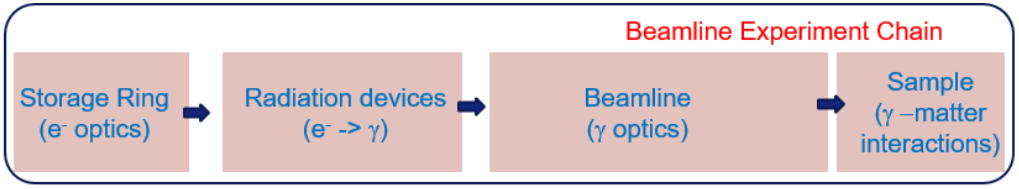
\includegraphics[width=14cm]{FIGURES/chain0.png}
\caption{Schematic workflow of a synchrotron experiment where simulations cover the electron beam, the photon source, the beamline and finally the interaction of the photon beam with the samples.}
\label{figChain0}
\end{figure}

We are conscient of the complexity, dimension and difficulty of such complete simulation in particular if one thinks on the large variety of beamlines and experimental techniques in use. At present, the power of OASYS resides in presenting a modular environment to allow simulations along the complete chain. OASYS now includes powerful tools to make simulations of points 2 (photon sources) and 3 (beamline optics). The ability to be extended to cover the electron beam characteristics and also the interaction with samples is also present and some results are obtained. 

%===============================


% , retrieving the parameters of the electron beam, calculating the radiation from magnetic structure, then transporting and optimizing the photon beam and eventually including models for interaction with materials to get instrumental functions, study analyzers and detectors and perform ab-initio simulations to support experimental data analysis. 
% 
% Electron Beam, Photon Source, Beamline, Sample interaction, Data modeling and analyses. 
% 
% Most X-ray techniques are based on a signal determined by the convolution of physical effects introduced by the sample with the characteristics of the photon beam mainly due to the source and beamline optics. The latter is the so-called Instrumental Profile Function (Cheary et al., 2004; Zuev, 2006).
% 
% The ray-tracing approach can be used to ab initio calculate the instrumental function of a synchrotron radiation beamline. This has been successfully tested with an X-ray powder diffraction (XRPD) beamline (Rebuffi and Scardi, 2014) used for line profile analysis, where complete control of the diffracted signal is necessary (Scardi et al., 2010). The synchrotron beam shape, divergence and energy distributions that result from the source characteristics and beamline optics contribute to broaden the diffraction peaks of the recorded diffractograms. The peak width dependence versus the 2θ angle (Caglioti et al., 1958; Sabine, 1987) is usually parameterized by Caglioti's equation (Scardi et al., 1994), where the full width at half-maximum (FWHM) of the instrumental peak profiles represented as pseudo-Voigt curves has the form FWHM(θ) = [W + Vtanθ + Utan2θ]1/2, where W, V and U are Caglioti's parameters and θ is the diffraction angle.
% 
% A special widget representing XRPD samples (see Fig. 7) in a capillary holder simulates the diffracted photon beam created by the interaction of the photon beam generated by SHADOW with a capillary filled by a crystalline material. The simulation takes into account not only the diffraction law but also the absorption of the photons by the sample material and the sample holder (that can be a source of considerable aberrations). Then, diffracted rays are traced onto the detector and other possible optical elements. The widget computes Caglioti's parameters fitting a pseudo-Voigt at every simulated diffraction peak.


\section{OASYS MECHANISM (CANVAS, WIDGETS AND ADD-ONS). KEY TECHNOLOGIES.}

A main feature of OASYS is to deliver a highly intuitive graphical interface provides high flexibility and rapidity for interactive simulations. Oasys presents an environment for synchrotron radiation virtual experiments. It is presented as a graphical environment (canvas) that can be populate with applications (widgets) which communicate among them. The applications come from different simulation packages interfaced into Oasys and called add-ons. The different add-ons are optional packages that can be installed or deinstalled depending on user's convinience. The interesting concept is that the users can add new add-ons depending on their needs. The canvas is populated with widgets that the user selects from the add-ons menus. The widgets are connected via ``wires'' that are channels for exchanging information. The kind of information is ``labelled'' in such a way that two widgets can be physically connected if one is capable to emit and the other is able to receive signals that are compatible, i.e., with the same label. In this way the user builds the simulation in a form of workflow containing widgets linked by wires. Every widget has a multiple functionality: it holds the input parameters, triggers a calculation or a data flow and displays results. All these functionality is embedded in a single window that opens by double-clicking the widget. Figure~\ref{figCanvas} presents an example of the canvas and a window from a widget. 
The flowchart concept of the application naturally permits to chain the elements of a virtual experiment. Configurations represented by a single or multiple widgets can be copied, duplicated and changed very quickly to compare multiple configurations. OASYS integrates in a synergetic way the most powerful calculation engines available, that are summarized in the next section. 

\begin{figure}[h]
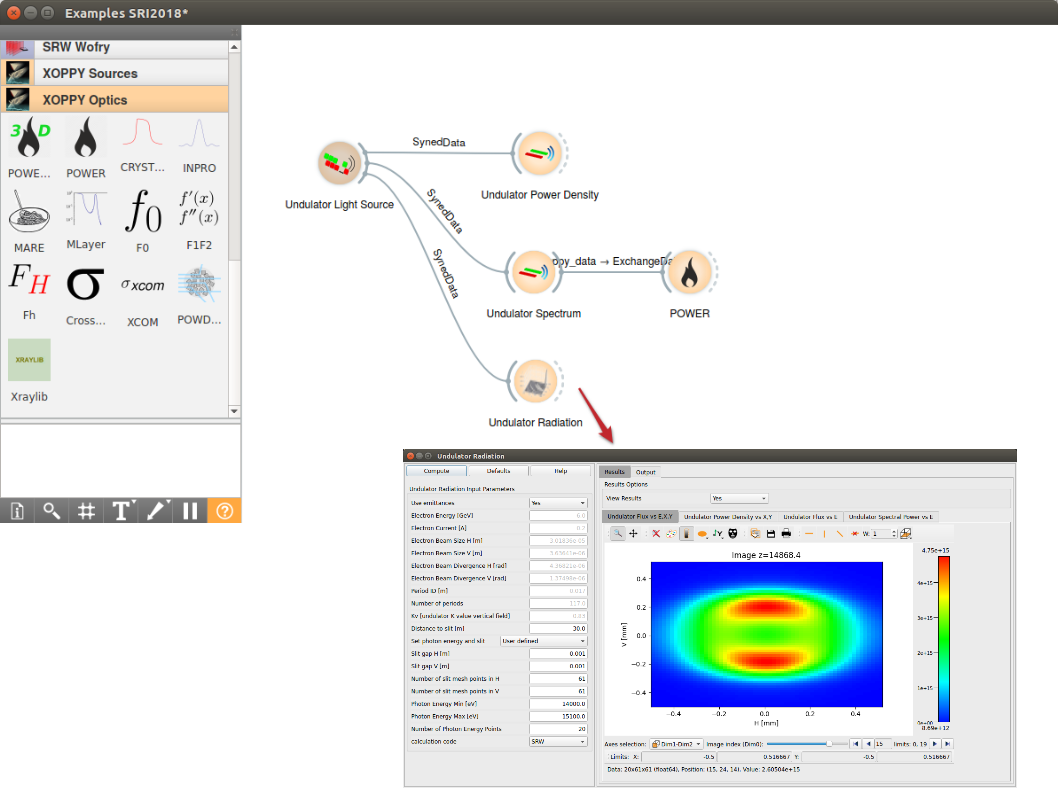
\includegraphics[width=14cm]{FIGURES/canvas.png}
\caption{OASYS application showing on the left area the menu zone containing the installed add-ons, the canvas with some widgets and connections, and a window with the parameters and results of the ``Undulator radiation'' application which computes the flux of an undulators as a function of the horizontal and vertical coordinates and photon energy.}
\label{figCanvas}
\end{figure}

In the initial phase of OASYS development, we first focused our attention on importing python-based APIs into its environment, but recently we dedicated our efforts on its final goal: to define a uniform and exchangeable description of the real world set up that is tailored to the synchrotron world and is still flexible enough to allow particularities for different algorithms and physical approaches. This is implemented by creating an object-oriented framework library, providing the glossary for the definition of light sources and optical components, together with a set of dedicated (so-called) widgets, the active elements of the OASYS graphical user interface (GUI) [11]. This common layer upon OASYS APIs has been called SYNED (SYNchrotron Elements Dictionary), and it is the base for allowing user to create workspaces with several APIs simulating the same beamline without data misalignment or redundancy, thus separating the description of the real world from details of the calculation algorithms and allowing users to easily benchmark their calculations by using different products for the same simulation.

OASYS goal is to become an integration platform where different software packages can communicate by sharing information and results, allowing the user to perform multi-application, complex analysis and simulations easily and safely. To achieve this goal, a careful planning on the technologies and right selections of the tools is necessary. The boundary conditions we imposed is to be open-source, work with open-source tools and be compatible with applications, libraries and packages developed in the academic context. For this reason Python has been selected as main language. It lives a very wide ecosystem with plenty of tools developed by a huge community. 

%================================




After implementing these common definitions and data structures, we work on the creation of a software platform able to combine different APIs, by exchanging data and calculation results. The final purpose is to optimize running different calculations and making comparisons of the results. The first integration framework library we developed is dedicated to wave optics and it is called WOFRY (Wave Optics FRamework in pYthon), a generalization (or abstraction) of a wavefront propagation software tool, combined with the SYNED definition of a synchrotron radiation beamline.








Existing OASYS API like ShadowOui [11] and the wavefront propagation tool WISE [12] and XOPPY (XOP [13] in PYthon) has been refactored to be compatible with SYNED. The SRW OASYS prototype API has been implemented according to both WOFRY and SYNED frameworks. UML [14] class diagrams, implementation details and examples of both framework are shown in the following paragraphs.

The ultimate purpose of OASYS is to integrate in a synergetic way the most powerful calculation engines available to perform virtual experiments in a synchrotron beamline, from the electron emission to the sample scattering. For X-ray Optics, OASYS integrates different simulation strategies via the implementation of adequate simulation tools (e.g. ray tracing and wave optics packages). It provides a language to make them to communicate by sending and receiving encapsulated data.

OASYS is a modern and user-friendly graphical environment for modelling X-ray experiments, where several top-level optical simulation tools have already been successfully integrated. We showed by examples how the OASYS environment allows the users to perform complex calculations in an intuitive and easy way, increasing the level of affordability of the optical design. OASYS and the available APIs (Add-Ons) is continuously developed since 2013 and upgraded both in term of number of functionalities and in robustness.




OASYS is fully based on the software Orange [2], developed at the University of Ljubljana (Slovenia), which is the high level workflow engine that provides the interaction with the user and communication mechanisms. Orange is a Python-based, comprehensive, component-based framework for data mining and machine learning users and developers. Orange is designed to simplify the assembly of data analysis workflows and crafting of data mining approaches from a combination of existing components. 

% OASYS is written in Python 3.4 and relies on PyQt 5.8.2 [3] for the GUI appearance. Complementing the Orange workflow infrastructure, OASYS graphs and plots are based on the library silx [4]. X-ray-matter interaction cross sections and scattering functions are obtained from xraylib [5], used for most optical calculations.
% 
% The JSON integration as exchange format.
% 
% Remote access (SYNED-JSON, DABAM, X-RAY-SERVER)
% 
% PHYSICS: xraylib, scipy [codata] 
% 
% GRAPHICS: silx


\begin{figure}[h]
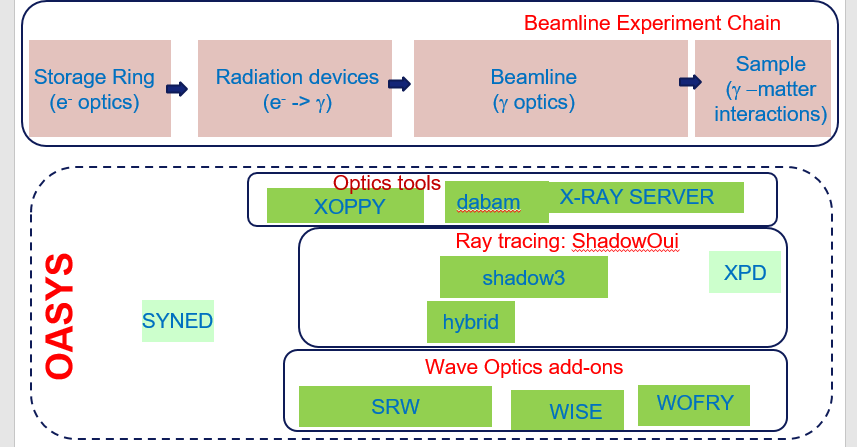
\includegraphics[width=14cm]{FIGURES/chain.png}
\caption{Effect of grazing angle (20, 25, 30 and 40 mrad, from top row to botom row) for systems using paraboloid mirrors. The source horizontal divergence is $\Upsilon_h$=10 mrad}
\label{figGrazing}
\end{figure}


\section{THE OPTICS TOOLS}

OASYS integrates different simulation strategies via the implementation of adequate simulation tools for X-ray Optics (e.g. ray tracing and wave optics packages). 

\subsection{The toolboxes}

\subsection{Optics for incoherent optics. Ray-tracing and its environment.}

The first step before the construction of any X-ray system, such as a synchrotron beamline, is an
accurate conceptual design of the optics. The beam should be transported to a given image plane
(usually the sample position) and its characteristics should be adapted to the experimental
requirements, in terms of flux, energy bandwidth, beam divergence, focal size, time structure, etc.
Today, optical design relies more and more on computer simulation and optimization. These programs
can be divided in two groups, those based on the propagation of rays along well defined optical paths,
and those that propagate waves. The first ones are based on geometrical optics whereas the second
ones rely on physical or wave optics. Some optical effects are better described by a geometrical model
(sometimes extended by associating electric fields to each ray) like aberrations, errors in the optical
surfaces, beam dimensions, role of critical angle in beam intensity, etc., whereas others, like
interference and diffraction, are better explained using a wave model. Wave optics methods are
computationally more expensive, as usually one has to finely grid the phase space. Hybrid methods
permitting to switch from one description to another and vice versa would be ideal. The present trend
[1] is the co-existence of software tools that allow treating the same system from two points of view.
The integration of these two approaches into a single computer environment is a challenge that will
certainly be developed in the near future. This paper describes the recent developments in ray tracing,
mainly in connection with the SHADOW [2] code. At the end of the paper, some ideas of integration
of ray tracing and wave optics are discussed, and some collaborative effort is on progress. 

A hybrid method combining ray-tracing and wavefront propagation was recently developed for X-ray optics simulation and beamline design optimization. One major application of the hybrid method is its ability to assess the effects of figure errors on the performance of focusing mirrors. In the present work, focusing profiles of mirrors with different figure errors are simulated using three available wave optics methods: the hybrid code based on the Fourier optics approach, the stationary phase approximation and a technique based on the direct Fresnel-Kirchhoff diffraction integral. The advantages and limitations of each wave optics method are discussed. We also present simulations performed using the figure errors of an elliptical cylinder mirror measured at APS using microstitching interferometry. These results show that the hybrid method provides accurate and quick evaluation of the expected mirror performance making it a useful tool for designing diffraction-limited focusing beamlines.

An open-source database containing metrology data for X-ray mirrors is presented. It makes available metrology data (mirror heights and slopes profiles) that can be used with simulation tools for calculating the effects of optical surface errors in the performances of an optical instrument, such as a synchrotron beamline. A typical case is the degradation of the intensity profile at the focal position in a beamline due to mirror surface errors. This database for metrology (DABAM) aims to provide to the users of simulation tools the data of real mirrors. The data included in the database are described in this paper, with details of how the mirror parameters are stored. An accompanying software is provided to allow simple access and processing of these data, calculate the most usual statistical parameters, and also include the option of creating input files for most used simulation codes. Some optics simulations are presented and discussed to illustrate the real use of the profiles from the database.


\subsection{Optics for coherent optics. Wavefront propagation.}

\subsection{Towards simulations for partial coherence optics}

\section{OASYS availability, customization, extensibility}

% \section{FIRST-ORDER HEADING}
% This is an example of dummy text. This is an example of dummy text. This is an example of dummy text.
% This is an example of dummy text. This is an example of dummy text. This is an example of dummy text.
% 
% This is the paragraph spacing that occurs when you use the [ENTER] key.
% 
% % Head 2
% \subsection{Second-Order Heading}
% This is an example of dummy text. This is an example of dummy text. This is an example of dummy text.
% This is an example of dummy text. This is an example of dummy text. This is an example of dummy text.
% This is an example of dummy text. This is an example of dummy text. This is an example of dummy text.
% This is an example of dummy text. This is an example of dummy text. This is an example of dummy text.
% 
% 
% % Head 3
% \subsubsection{Third-Order Heading}
% Physical data should be quoted with decimal points and negative exponents (e.g., 25.8 J K$^{-1}$ mol$^{-1}$), and arranged as follows where possible: mp/bp 20$^{\circ}$C; [$\alpha$]D20 $=$ $-$13.5 ($c = 0.2$, acetone) (please also give units for [$\alpha$] and $c$, usually deg cm$^3$ g$^{-1}$ dm$^{-1}$ and g cm$^{-3}$, respectively); 1H NMR (400 MHz, DMSO-$d_6$, $\delta$): 7.15 (s, 2H, Ar H), 1.3 (q, $J = 8$ Hz, 2H; CH$_2$), 0.9 (t, $J = 8$ Hz, 3H; CH$_3$); $^{13}$C NMR (100 MHz, CDCl$_3$, δ): 175.4 (C$=$O), 156.5 (C4); IR (KBr): $\nu = 2972$ (w), 2907 (w), \ldots, 1026 (s; $\nu_{\rm as}$(SiOSi)), 971 ($\nu_{\rm s}$), $\ldots$, 666 (w; $\nu_{\rm s}$(SiOSi)), \ldots, 439 (m), 401 cm$^{-1}$ (m); UV-vis ($n$-hexane): $\lambda_{\max}$ ($\varepsilon$) $=$ 320 (5000), 270 nm (12000); EIMS $m/z$ (\%): 108 (20) [M$^+$], 107 (60) [M$^+$ $-$ H], 91 (100) [C$_7$H$_7^+$]; HRMS (ESI) $m/z$: [M $+$ H]$^+$ calcd for C$_{21}$H$_{38}$N$_{4}$O$_{6}$S, 475.2591; found, 475.2593. Anal. calcd for C$_{45}$H$_{28}$N$_{4}$O$_{7}$: C 62.47, H 3.41, N 6.78; found: C 62.27, H 3.46, N 6.80.
% 
% % enumerate
% \noindent Numbered lists may also be included and should look like this:
% 
% \begin{enumerate}
% \item This is an example of numbered listing.
% \item This is an example of numbered listing. This is an example of numbered listing.
% \item This is an example of numbered listing.
% \item This is an example of numbered listing. This is an example of numbered listing.
% \item This is an example of numbered listing.
% \item This is an example of numbered listing. This is an example of numbered listing.
% \end{enumerate}
% 
% \noindent Bulleted lists may be included and should look like this:
% % itemize
% 
% \begin{itemize}
% \item This is an example of bulleted listing.
% \item This is an example of bulleted listing. This is an example of bulleted listing.
% \item This is an example of bulleted listing.
% \item This is an example of bulleted listing. This is an example of bulleted listing.
% \item This is an example of bulleted listing.
% \end{itemize}
% 
% \noindent This is an example of single line numbered equation.
% \begin{equation}
% \frac{d[F_1]}{d\omega_2} = SAm_2\cos\omega,\frac{d[F_1]}{d\omega_3}= SAm_2\cos\omega.
% \end{equation}
% 
% This is an example of a multiline numbered equation.
% % Numbered multiple equation
% \begin{eqnarray}
% p_{t_{10,1}}&=&\left(\frac{N_{cu}^2}{ N_c ^2}\right)\left(\frac{N_{ar}^2}{N_a^2}\right)\left(\frac{N_{ar}-1}{N_{ar}}\right),\\
% p_{t_{10,2}}&=&\left(\frac{N_{cu}^2}{ N_c ^2}\right)\left(\frac{N_{ar}}{N_a^2}\right).
% \end{eqnarray}
% 
% % Unnumbered equation
% %% \begin{eqnarray*}
% %% {\rm ((Multi\ Equation\ Unnumbered))}\\
% %% {\rm ((Multi\ Equation\ Unnumbered))}\\
% %% {\rm ((Multi\ Equation\ Unnumbered))}
% %% \end{eqnarray*}
% %% this is an example of dummy text.
% % Unnumbered equation
% %% \[
% %% {\rm ((Single\ Equation\ Unnumbered))}
% %% \]
% %% this is an example of dummy text.
% For more on equations, please refer to the guide.
% 
% \section{OTHER SPECIFICATIONS (FIRST LEVEL HEADING)}
% Figures, tables, and equations must be inserted in the text and may not be grouped at the end of the paper. Important: A miscount of figures, tables, or equations may result from revisions. Please double check the numbering of these elements before you submit your paper to your proceedings editor.
% 
% \subsection{Figures (Second Level Heading)}
% If you need to arrange a number of figures, a good tip is to place them in a table, which gives you additional control of the layout. Leave a line space between your figure and any text above it, like this one:
% 
% % Figure
% \begin{figure}[h]
%   \centerline{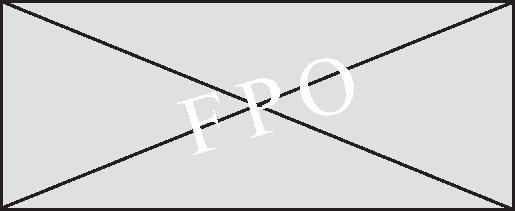
\includegraphics[width=150pt]{FIGURES-TMP/fig_1}}
%   \caption{To format a figure caption use the \LaTeX template style: Figure Caption. The text ``FIGURE 1,'' which labels the caption, should be bold and in upper case. If figures have more than one part, each part should be labeled (a), (b), etc. Using a table, as in the above example, helps you control the layout.}
% \end{figure}
% 
% \begin{sidewaysfigure}
%   \centerline{
\includegraphics[width=500pt]{FIGURES-TMP/fig_2}}
%   \caption{To format a figure caption use the \LaTeX template style: Figure Caption. The text ``FIGURE 2,'' which labels the caption, should be bold and in upper case. If figures have more than one part, each part should be labeled (a), (b), etc. Using a table, as in the above example, helps you control the layout.}
% \end{sidewaysfigure}
% 
% Cite all figures in the text consecutively. The word ``Figure'' should be spelled out if it is the first word of the sentence and abbreviated as ``Fig.'' elsewhere in the text. Place the figures as close as possible to their first mention in the text at the top or bottom of the page with the figure caption positioned below the figure, all centered. Figures must be inserted in the text and may not follow the Reference section. Set figure captions in 9 point size, Times Roman font. Type the word ``FIGURE 1.'' in bold uppercase, followed by a period.\footnote{This is an example of a footnote.}
% 
% 
% Authors are welcome to use color figures within their article. For online publication, there are no costs added for color figures. However, for printed proceedings (if requested by your conference organizer), there is an additional cost. Please consult directly with your conference organizer. If your conference organizer has asked AIP Publishing to produce printed copies (many ask AIP Publishing for online-only publication), then all figures will be printed in black-and-white unless you make specific arrangements with your organizer(s) to include color figures in your article and pay to them the associated fee(s) they request. We advise that many color figures can be printed in black-and-white with no loss of information; however, some figures do lose information when reproduced in black-and-white. Check your figure legends carefully and, if your figures are to be printed in black-and-white, remove from your text/descriptions any references to color.
% 
% 
% \subsection{Tables (Second Level Heading)}
% Due to the wide range and complexity of tables, we simply offer an example for guidance. Please follow the style for Table \ref{tab:a} (and figure) captions.
% 
% % Table
% \begin{table}[h]
% \caption{To format a table caption, use the \LaTeX template style: Table Caption. The text ``{\bf TABLE 1,}'' which labels the caption, should be bold and all letters capitalized. Center this text above the table. Tables should have top and bottom rules, and a rule separating the column heads from the rest of the table only.}
% \label{tab:a}
% \tabcolsep7pt\begin{tabular}{lcccc}
% \hline
%   & \tch{1}{c}{b}{Single\\ outlet}  & \tch{1}{c}{b}{Small\\ multiple\tabnoteref{t1n1}}  & \tch{1}{c}{b}{Large\\ multiple}  & \tch{1}{c}{b}{Total}   \\
% \hline
% 1982 & 98 & 129 & 620    & 847\\
% 1987 & 138 & 176 & 1000  & 1314\\
% 1991 & 173 & 248 & 1230  & 1651\\
% 1998 & 200 & 300 & 1500\tabnoteref{t1n2}  & 2000\\
% \hline
% \end{tabular}
% \tablenote[t1n1]{This is an example of first tablenote entry. This is an example of first tablenote entry.}
% \tablenote[t1n2]{This is an example of second tablenote entry.}
% \end{table}
% 
% \subsection{Font Embedding (Second Level Heading)}
% As the author and creator of your article PDF, you have the most intimate knowledge of exactly what the PDF should display. We ask all authors to carefully check their article PDF prior to submission. Perform visual inspections to detect subtle font errors and ensure that all fonts are embedded. With the wide range of tools and software that authors use to create PDFs, and the number of devices and platforms that readers use to view/print them, font embedding by authors is not only ``nice-to-have'', it is essential. 
% 
% \subsubsection{Why Should I Care About Font Embedding? (Third Level Heading)}
% Embedding fonts into your PDF file is critically important for two reasons:
% \begin{itemize}
% \item Commercial printing companies are unable to print PDFs without the correct fonts embedded.
% \item To ensure that your online article PDF file displays and prints correctly for everyone who wants to read your work.
% \end{itemize}
% 
% Readers of scientific articles use an ever-increasing range of devices and applications to access, view, and print PDFs  from smart phones and tablets to desktop computers running any one of a number of operating systems. To ensure that readers of  your article can display and print it correctly, it is important for your article's PDF file to be truly portable. Your PDF file needs to be fully ``self-contained.''%\vfill\pagebreak
% 
% \section{FINAL KEY POINTS TO CONSIDER (FIRST LEVEL HEADING)}
% Here are the main points you need to follow (the AIP Publishing author template packages contain comprehensive guidance):
% 
% \begin{itemize}
% \item Write and prepare your article using the AIP Publishing template.
% \item Create a PDF file of your paper (making sure to embed all fonts).
% \item Send the following items to your conference organizer:
% \begin{itemize}
% \item PDF file of your paper
% \item Signed Copyright Transfer Agreement
% \item (If it applies) Copies of any permissions to re-use copyrighted materials in your article (e.g., figures from books/journals)
% \end{itemize}
% \end{itemize}
% 
% 
% 
% % Sections that will go in second font
% 
% % Acknowledgement
% \section{ACKNOWLEDGMENTS}
% The reference section will follow the ``Acknowledgment'' section.  References should be numbered using Arabic numerals followed by a period (.) as shown below, and should follow the format in the below examples.
% 
% % References
% 
% % [1] Rebuffi, L and Sanchez del Rio, M. "OASYS (OrAnge SYnchrotron Suite): an open-source graphical environment for x-ray virtual experiments”, Proc. SPIE 10388, 103880S (2017)
% % [2] Rebuffi, L and Sanchez del Rio, M. "ShadowOui: A new visual environment for X-ray optics and synchrotron beamline simulations”, J. Synchrotron Rad. 23 (2016)
% % [3] Chubar, O., Elleaume, P. “Accurate and Efficient Computation of Synchrotron Radiation In The Near Field Region,” Proceedings of the EPAC98 Conference, 22–26 June 1998, 1177–1179 (1998).
% % [4] Demšar, J., Curk, T. and Erjavec, A. “Orange: Data Mining Toolbox in Python,” Journal of Machine Learning Research 14, 2349–2353 (2013). 


%\nocite{*}
\bibliography{references}%
\bibliographystyle{aipnum-cp}%



\end{document}
